\documentclass{standalone}
\usepackage{tikz}
\usetikzlibrary{patterns, positioning}
\usepackage[sfdefault]{ClearSans} %% option 'sfdefault' activates Clear Sans as the default text font
\usepackage[T1]{fontenc}

\begin{document}
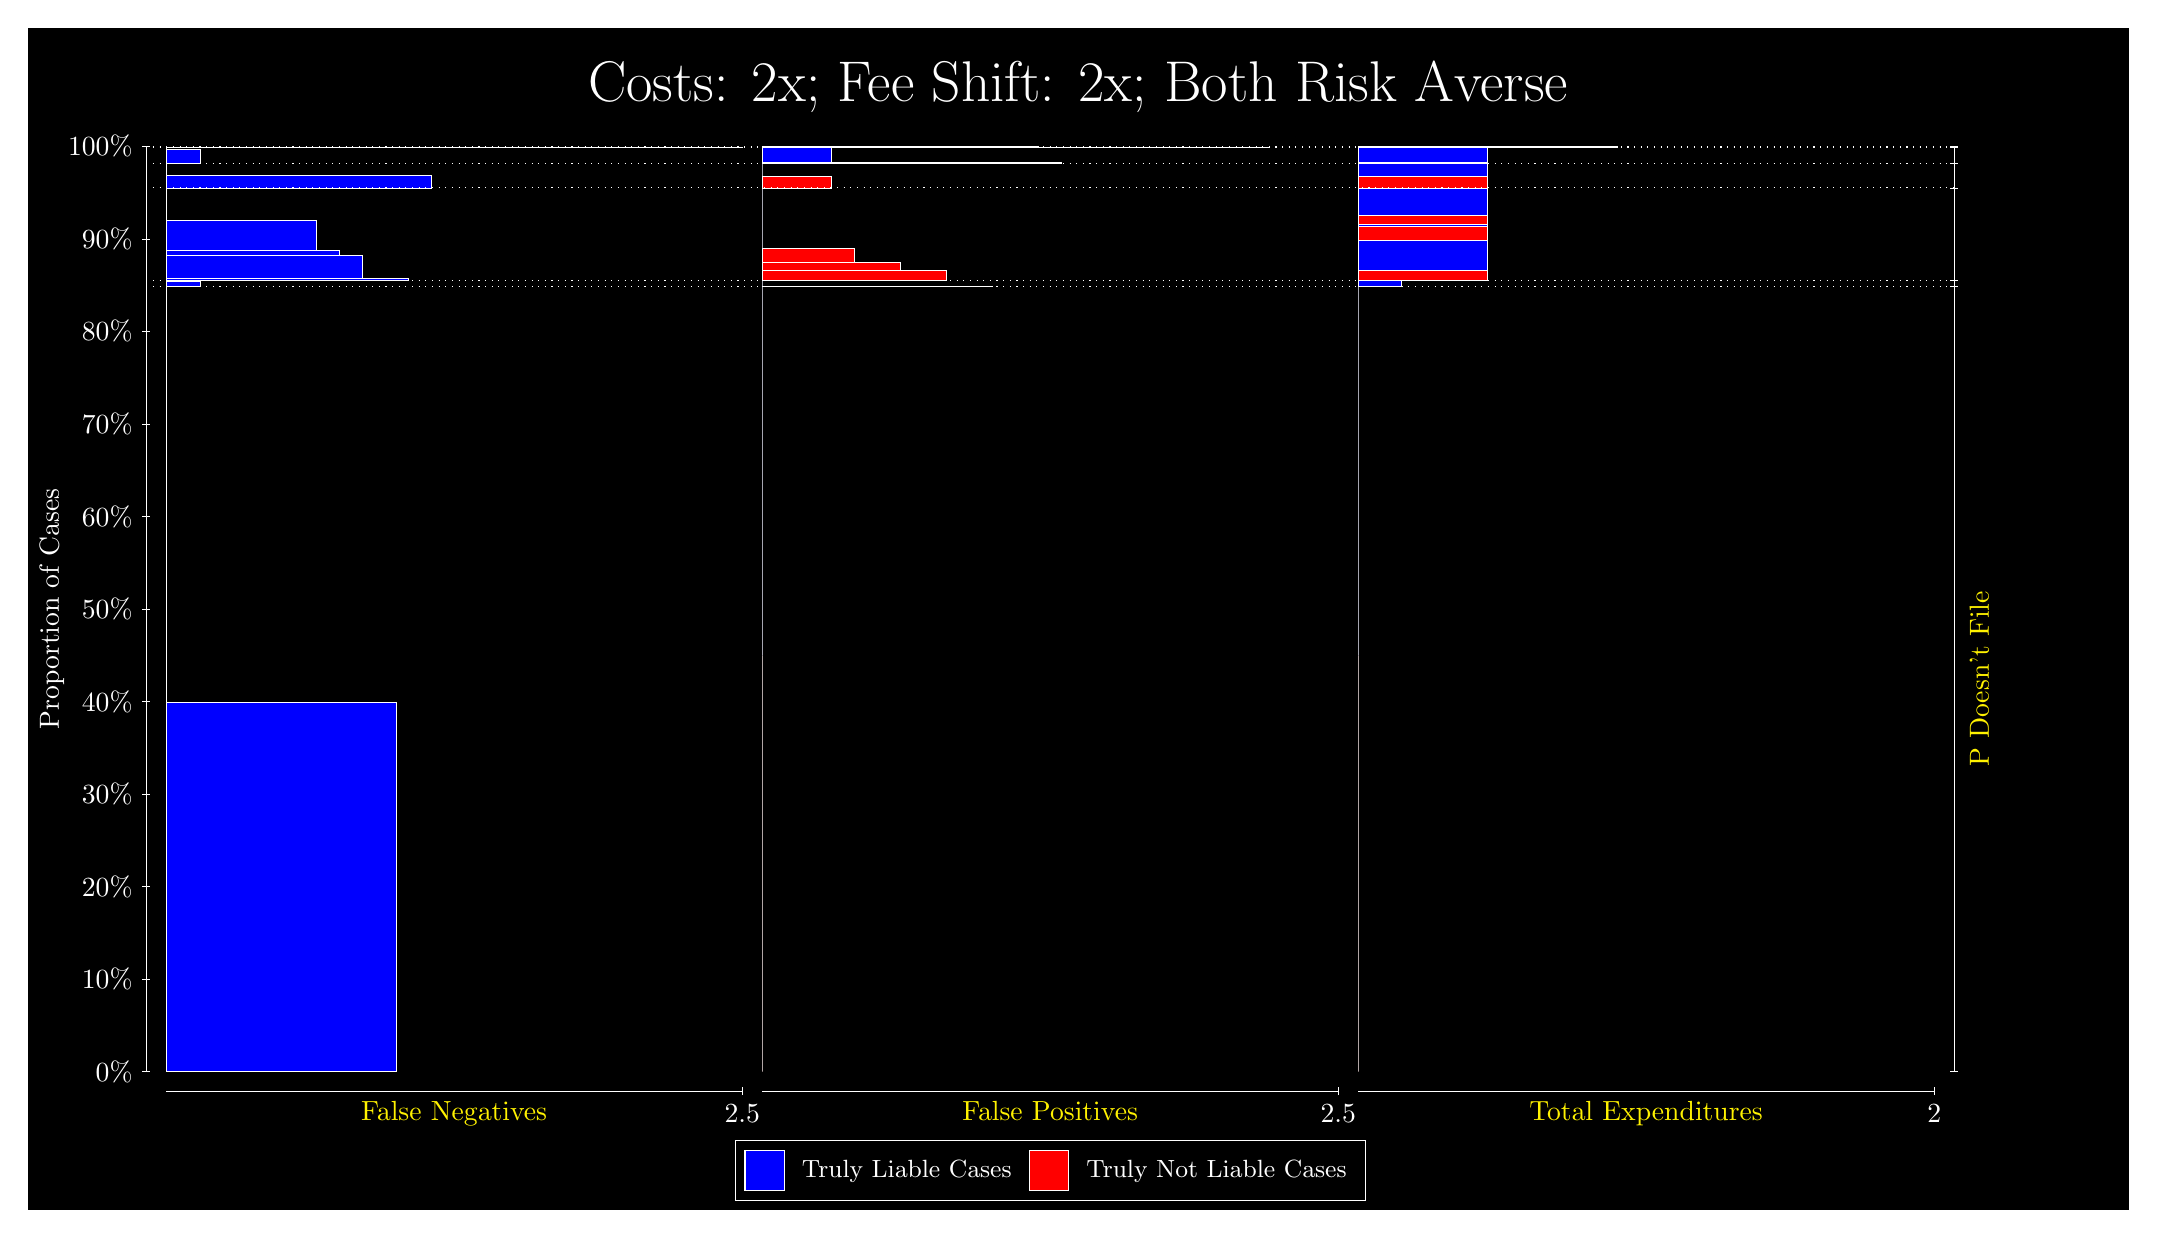
\begin{tikzpicture}
\draw[fill=black] (0,0) rectangle (26.667,15);
\draw[text=white] (0,13.5) rectangle (26.667,15) node[midway] {\huge Costs: 2x; Fee Shift: 2x; Both Risk Averse};
\draw[white, very thin] (1.5,1.75) -- (1.5,13.5);
\node[rotate=90, text=white, anchor=center] at (0.3, 7.625) {Proportion of Cases};
\draw[white, very thin] (1.45,1.75) -- (1.55,1.75);
\node[text=white, anchor=east] at (1.45, 1.75) {0\%};
\draw[white, very thin] (1.45,2.925) -- (1.55,2.925);
\node[text=white, anchor=east] at (1.45, 2.925) {10\%};
\draw[white, very thin] (1.45,4.1) -- (1.55,4.1);
\node[text=white, anchor=east] at (1.45, 4.1) {20\%};
\draw[white, very thin] (1.45,5.275) -- (1.55,5.275);
\node[text=white, anchor=east] at (1.45, 5.275) {30\%};
\draw[white, very thin] (1.45,6.45) -- (1.55,6.45);
\node[text=white, anchor=east] at (1.45, 6.45) {40\%};
\draw[white, very thin] (1.45,7.625) -- (1.55,7.625);
\node[text=white, anchor=east] at (1.45, 7.625) {50\%};
\draw[white, very thin] (1.45,8.8) -- (1.55,8.8);
\node[text=white, anchor=east] at (1.45, 8.8) {60\%};
\draw[white, very thin] (1.45,9.975) -- (1.55,9.975);
\node[text=white, anchor=east] at (1.45, 9.975) {70\%};
\draw[white, very thin] (1.45,11.15) -- (1.55,11.15);
\node[text=white, anchor=east] at (1.45, 11.15) {80\%};
\draw[white, very thin] (1.45,12.325) -- (1.55,12.325);
\node[text=white, anchor=east] at (1.45, 12.325) {90\%};
\draw[white, very thin] (1.45,13.5) -- (1.55,13.5);
\node[text=white, anchor=east] at (1.45, 13.5) {100\%};

\draw[white, very thin] (24.457,1.75) -- (24.457,13.5);
\draw[white, very thin] (24.407,1.75) -- (24.507,1.75);
\node[anchor=west] at (24.407, 1.75) {};
\draw[white, very thin] (24.407,11.719) -- (24.507,11.719);
\node[anchor=west] at (24.407, 11.719) {};
\draw[white, very thin] (24.407,11.8) -- (24.507,11.8);
\node[anchor=west] at (24.407, 11.8) {};
\draw[white, very thin] (24.407,12.972) -- (24.507,12.972);
\node[anchor=west] at (24.407, 12.972) {};
\draw[white, very thin] (24.407,13.282) -- (24.507,13.282);
\node[anchor=west] at (24.407, 13.282) {};
\draw[white, very thin] (24.407,13.488) -- (24.507,13.488);
\node[anchor=west] at (24.407, 13.488) {};
\draw[white, very thin] (24.407,13.492) -- (24.507,13.492);
\node[anchor=west] at (24.407, 13.492) {};
\draw[white, very thin] (24.407,13.5) -- (24.507,13.5);
\node[anchor=west] at (24.407, 13.5) {};

\draw[white, very thin, fill=blue] (1.75,1.75) rectangle (4.6775,6.4348);
\draw[white, very thin, fill=red] (1.75,6.4348) rectangle (1.75,11.719);
\draw[white, very thin, fill=blue] (1.75,11.719) rectangle (2.1891,11.792);
\draw[white, very thin, fill=red] (1.75,11.792) rectangle (1.75,11.8);
\draw[white, very thin, fill=blue] (1.75,11.8) rectangle (4.8239,11.827);
\draw[white, very thin, fill=blue] (1.75,11.827) rectangle (4.2384,12.122);
\draw[white, very thin, fill=blue] (1.75,12.122) rectangle (3.9457,12.176);
\draw[white, very thin, fill=blue] (1.75,12.176) rectangle (3.6529,12.566);
\draw[white, very thin, fill=red] (1.75,12.566) rectangle (1.75,12.972);
\draw[white, very thin, fill=blue] (1.75,12.972) rectangle (5.1167,13.129);
\draw[white, very thin, fill=red] (1.75,13.129) rectangle (1.75,13.282);
\draw[white, very thin, fill=blue] (1.75,13.282) rectangle (2.1891,13.468);
\draw[white, very thin, fill=red] (1.75,13.468) rectangle (1.75,13.488);
\draw[white, very thin, fill=blue] (1.75,13.488) rectangle (9.0689,13.49);
\draw[white, very thin, fill=red] (1.75,13.49) rectangle (1.75,13.492);
\draw[white, very thin, fill=red] (1.75,13.492) rectangle (1.75,13.493);
\draw[white, very thin, fill=blue] (1.75,13.493) rectangle (1.75,13.5);
\draw[white, very thin, fill=red] (9.3189,1.75) rectangle (9.3189,7.0345);
\draw[white, very thin, fill=blue] (9.3189,7.0345) rectangle (9.3189,11.719);
\draw[white, very thin, fill=red] (9.3189,11.719) rectangle (12.246,11.728);
\draw[white, very thin, fill=blue] (9.3189,11.728) rectangle (9.3189,11.8);
\draw[white, very thin, fill=red] (9.3189,11.8) rectangle (11.661,11.921);
\draw[white, very thin, fill=red] (9.3189,11.921) rectangle (11.368,11.926);
\draw[white, very thin, fill=red] (9.3189,11.926) rectangle (11.075,12.032);
\draw[white, very thin, fill=red] (9.3189,12.032) rectangle (10.49,12.206);
\draw[white, very thin, fill=blue] (9.3189,12.206) rectangle (9.3189,12.972);
\draw[white, very thin, fill=red] (9.3189,12.972) rectangle (10.197,13.125);
\draw[white, very thin, fill=blue] (9.3189,13.125) rectangle (9.3189,13.282);
\draw[white, very thin, fill=red] (9.3189,13.282) rectangle (13.125,13.302);
\draw[white, very thin, fill=blue] (9.3189,13.302) rectangle (10.197,13.488);
\draw[white, very thin, fill=red] (9.3189,13.488) rectangle (9.3189,13.49);
\draw[white, very thin, fill=blue] (9.3189,13.49) rectangle (9.3189,13.492);
\draw[white, very thin, fill=red] (9.3189,13.492) rectangle (15.759,13.493);
\draw[white, very thin, fill=blue] (9.3189,13.493) rectangle (12.832,13.5);
\draw[white, very thin, fill=red] (16.888,1.75) rectangle (16.888,7.0345);
\draw[white, very thin, fill=blue] (16.888,7.0345) rectangle (16.888,11.719);
\draw[white, very thin, fill=red] (16.888,11.719) rectangle (17.437,11.728);
\draw[white, very thin, fill=blue] (16.888,11.728) rectangle (17.437,11.8);
\draw[white, very thin, fill=red] (16.888,11.8) rectangle (18.534,11.921);
\draw[white, very thin, fill=blue] (16.888,11.921) rectangle (18.534,12.311);
\draw[white, very thin, fill=red] (16.888,12.311) rectangle (18.534,12.484);
\draw[white, very thin, fill=blue] (16.888,12.484) rectangle (18.534,12.512);
\draw[white, very thin, fill=red] (16.888,12.512) rectangle (18.534,12.623);
\draw[white, very thin, fill=blue] (16.888,12.623) rectangle (18.534,12.972);
\draw[white, very thin, fill=red] (16.888,12.972) rectangle (18.534,13.125);
\draw[white, very thin, fill=blue] (16.888,13.125) rectangle (18.534,13.282);
\draw[white, very thin, fill=red] (16.888,13.282) rectangle (18.534,13.302);
\draw[white, very thin, fill=blue] (16.888,13.302) rectangle (18.534,13.488);
\draw[white, very thin, fill=red] (16.888,13.488) rectangle (20.181,13.49);
\draw[white, very thin, fill=blue] (16.888,13.49) rectangle (20.181,13.492);
\draw[white, very thin, fill=red] (16.888,13.492) rectangle (20.181,13.493);
\draw[white, very thin, fill=blue] (16.888,13.493) rectangle (20.181,13.5);
\draw[white, dotted] (1.5,11.719) -- (24.457,11.719);
\draw[white, dotted] (1.5,11.8) -- (24.457,11.8);
\draw[white, dotted] (1.5,12.972) -- (24.457,12.972);
\draw[white, dotted] (1.5,13.282) -- (24.457,13.282);
\draw[white, dotted] (1.5,13.488) -- (24.457,13.488);
\draw[white, dotted] (1.5,13.492) -- (24.457,13.492);
\draw[white, very thin] (1.75,1.5) -- (9.0689,1.5);
\node[text=yellow, anchor=north] at (5.4094, 1.5) {False Negatives};
\draw[white, very thin] (9.0689,1.45) -- (9.0689,1.55);
\node[text=white, anchor=north] at (9.0689, 1.45) {2.5};

\draw[white, very thin] (9.3189,1.5) -- (16.638,1.5);
\node[text=yellow, anchor=north] at (12.978, 1.5) {False Positives};
\draw[white, very thin] (16.638,1.45) -- (16.638,1.55);
\node[text=white, anchor=north] at (16.638, 1.45) {2.5};

\draw[white, very thin] (16.888,1.5) -- (24.207,1.5);
\node[text=yellow, anchor=north] at (20.547, 1.5) {Total Expenditures};
\draw[white, very thin] (24.207,1.45) -- (24.207,1.55);
\node[text=white, anchor=north] at (24.207, 1.45) {2};

\node[text=yellow, centered, rotate=90] at (24.777, 6.7347) {P Doesn't File};







\draw (12.978300999999998,1.5) node[draw=none] (baseCoordinate) {};
\begin{scope}[align=center]
        \matrix[scale=0.5, draw=white, below=0.5cm of baseCoordinate, nodes={draw}, column sep=0.1cm]{
            \node[rectangle, draw, minimum width=0.5cm, minimum height=0.5cm, fill=blue] {}; &
            \node[draw=none, font=\small, text=white] (B) {Truly Liable Cases}; &
            \node[rectangle, draw, minimum width=0.5cm, minimum height=0.5cm, fill=red] {}; &
            \node[draw=none, font=\small, text=white] (B) {Truly Not Liable Cases}; \\
            };
\end{scope}

\end{tikzpicture}
\end{document}